\documentclass[30pt, a0paper, portrait, margin=0mm, innermargin=15mm,
               blockverticalspace=15mm, colspace=15mm, subcolspace=8mm]{tikzposter} 

% Change font     
\renewcommand{\familydefault}{\sfdefault}

\definecolor{mycol}{HTML}{326E77}
\definecolorstyle{myColorStyle}{
  \colorlet{colorOne}{darkgray}
  \colorlet{colorTwo}{gray}
  \colorlet{colorThree}{gray}
}{
  % Background Colors
  \colorlet{backgroundcolor}{colorTwo!50}
  \colorlet{framecolor}{black}
  % Title Colors
  \colorlet{titlefgcolor}{black}
  \colorlet{titlebgcolor}{colorOne}
  % Block Colors
  \colorlet{blocktitlebgcolor}{mycol}
  \colorlet{blocktitlefgcolor}{white}
  \colorlet{blockbodybgcolor}{white}
  \colorlet{blockbodyfgcolor}{black}
  % Innerblock Colors
  \colorlet{innerblocktitlebgcolor}{white}
  \colorlet{innerblocktitlefgcolor}{black}
  \colorlet{innerblockbodybgcolor}{white}
  \colorlet{innerblockbodyfgcolor}{black}
  % Note colors
  \colorlet{notefgcolor}{black}
  \colorlet{notebgcolor}{white}
  \colorlet{notefrcolor}{white}
}

% LATEX PACKAGES
% --------------
  
\usepackage{graphicx}  % package for inserting images, including .pdf
\usepackage{adjustbox} % package for cropping images
\usepackage[colorlinks=true, urlcolor=red]{hyperref} % package for url and hyperlinks
\usepackage{wrapfig}
\usepackage{lmodern} %mix italic and bold
\usepackage{hyperref}% for url
\usepackage{authblk}
\usepackage{graphicx} 
\usepackage{caption}
\usepackage{mwe}
\usepackage[absolute]{textpos}
\usepackage{selinput}
\usepackage{multicol}
\usepackage{wrapfig,kantlipsum}
\SelectInputMappings{%
  Lcaron={Ľ}
}


% TITLE, AUTHORS, INSTITUTE
% -------------------------

\title{\textbf{\parbox{\linewidth}{\centering Reduced Eimeria and pinworms loads in hybrid mice of the European house mouse hybrid zone}}}

\author[1,2]{Alice~Balard}
\author[1,2]{Victor~Hugo~Jarqu\'{i}n-D\'{i}az}
\author[1]{Jenny~Jost}
\author[3]{Iva~Martincov\'{a}}
\author[3]{{Ľ}udov\'{i}t \v{D}ureje}
\author[3]{Jaroslav~Pi\`alek}
\author[4]{Milo\v{s}~Macholán}
\author[3]{Jo\"{e}lle~Go\"{u}y~de~Bellocq}
\author[3]{Stuart~J.E.~Baird}
\author[1,2]{Emanuel~Heitlinger}

\affil[1]{\large Institute for Biology. Department of Molecular Parasitology. Humboldt University Berlin (HU). Philippstr. 13, Haus 14, 10115, Berlin, Germany}
\affil[2]{\large Leibniz-Institut für Zoo- und Wildtierforschung (IZW) im Forschungsverbund Berlin e.V.. Alfred-Kowalke-Straße 17, 10315, Berlin, Germany}
\affil[3]{\large Research Facility Studenec, Institute of Vertebrate Biology, Czech Academy of Sciences, Kv\v{e}tn\'{a} 8, 603 65 Brno, Czech Republic}
\affil[4]{\large Laboratory of Mammalian Evolutionary Genetics, Institute of Animal Physiology and Genetics, Czech Academy of Sciences, Veveri 97, 60200 Brno, Czech Republic\vspace{-6ex}% reduce space
}



\makeatletter
\def\maketitle{\AB@maketitle}
\makeatother

% THEME SETTING
% -------------
\usetheme{Default}
\usecolorstyle{myColorStyle}
\useblockstyle{Basic}
\usebackgroundstyle{Empty}
\usetitlestyle{Empty}

% Increase caption size
\usepackage{blindtext}
\makeatletter
\renewenvironment{tikzfigure}[1][]{
  \def \rememberparameter{#1}
  \vspace{10pt}
  \refstepcounter{figurecounter}
  \begin{center}
  }{
    \ifx\rememberparameter\@empty
    \else %nothing
    \\[5pt]
    {\large Fig.~\thefigurecounter: \rememberparameter}
    \fi
  \end{center}
}
\makeatother

% HEAD
% ----

\begin{document}
\maketitle

% Context
% ----

\block{General}
{
	\begin{itemize}
    \item Parasite models: 
	    \begin{itemize}
	  		\item \textit{Eimeria} spp., obligate intracellular parasite (Apicomplexa: Coccidia). \textbf{High impact on host health expected}
	  		\item Pinworms (\textit{Aspiruluris tetraptera} and \textit{Syphacia obvelata}). \textbf{Low impact on host health expected}
	    \end{itemize}
	  \item Host model: \textit{Mus musculus domesticus}, \textit{Mus musculus musculus} and their hybrids	
	  \item Aim of the study: \newline
\textbf{Investigating hybrid susceptibility/resistance of house mice to parasites presenting different pathogenicity, using prevalence and intensity data throughout the European house mouse hybrid zone}
  \end{itemize}
}	

% MATANDMET
% ----

% playing with multicolumn text
\block{Material \& Methods}{
  \begin{multicols*}{2}
    \begin{itemize}
 \item Sampling 660 mice over 4 years; Host genotyping (4-14 diagnostic markers) on a 0 to 1 scale (50/50 hybrids = 0.5)
 \item \textit{Eimeria} load estimated by quantitative PCR 
 \item Pinworm (\textit{Aspiculuris tetraptera} and \textit{Syphacia obvelata}) load estimated by count
 \item Modellisation of parasite load along hybridization index, test hybrid effect
 \item Logistic regression presence/absence of parasite in direction of the hybrid zone center
 \item Body condition (residuals body length/body weight) between infected/non infected + along gradient of hybridicity
      \end{itemize}
    \begin{tikzfigure}[Map of sub species separation in our sampling area]
            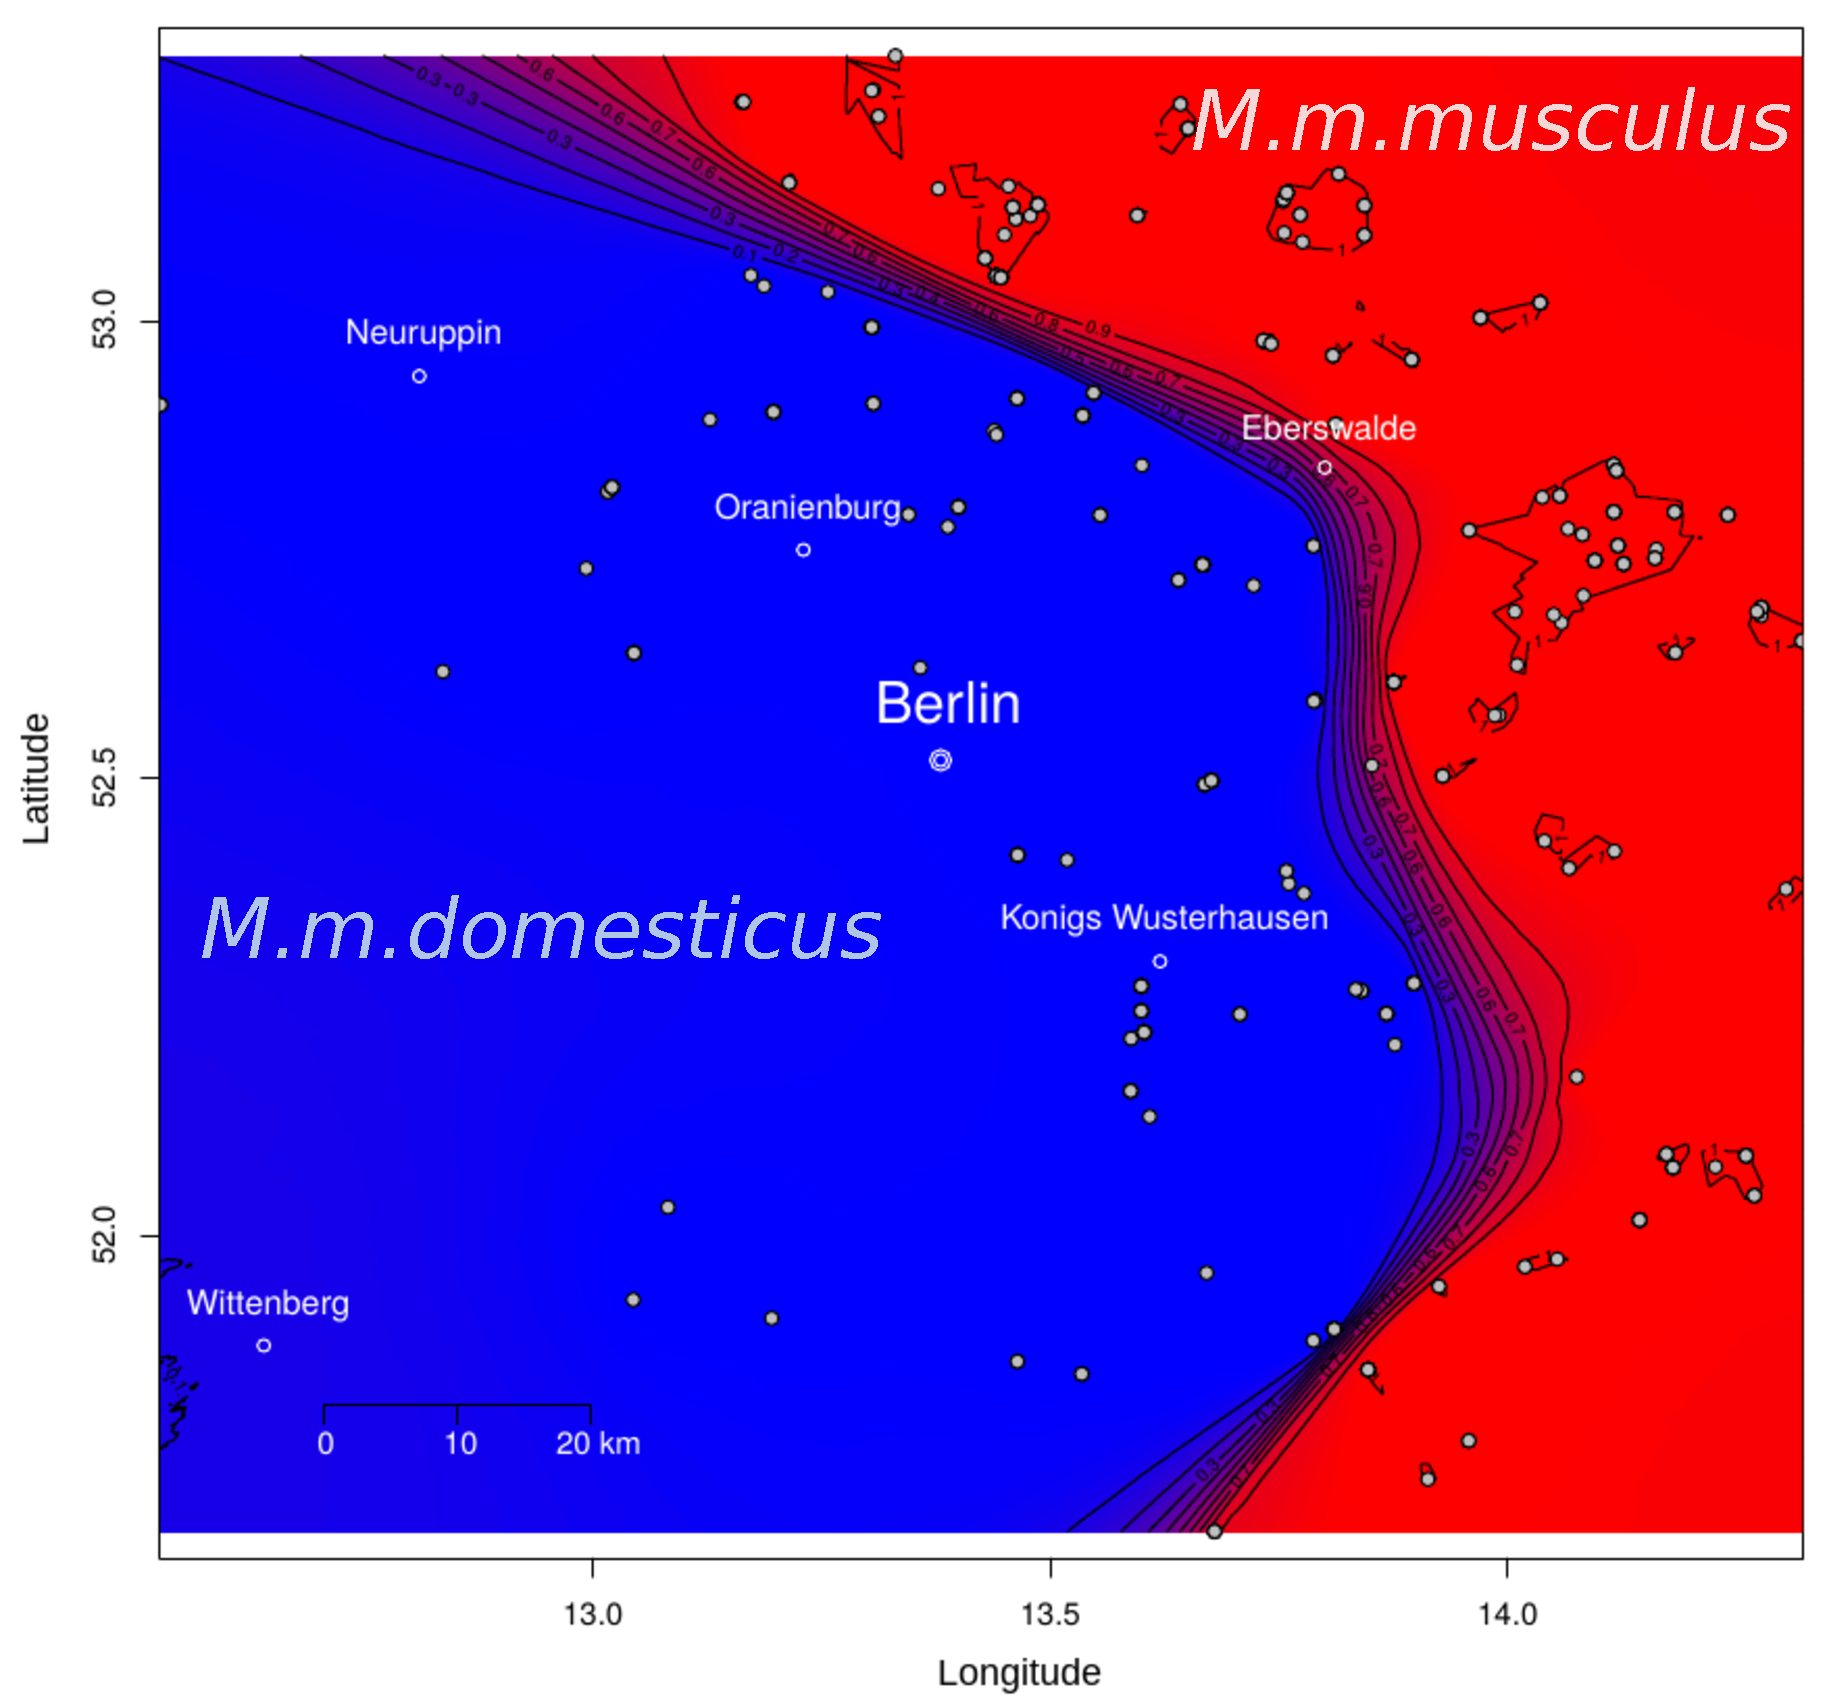
\includegraphics[scale=0.5]{Figure1.pdf}
    \end{tikzfigure}  \end{multicols*}
}

% Results: parasite load
% -------

\block{Results: \textit{Eimeria} spp. and pinworm load lower in hybrids than in parental mice}
      {
      \begin{multicols*}{2}
      
      \begin{tikzfigure}[Eimeria]
        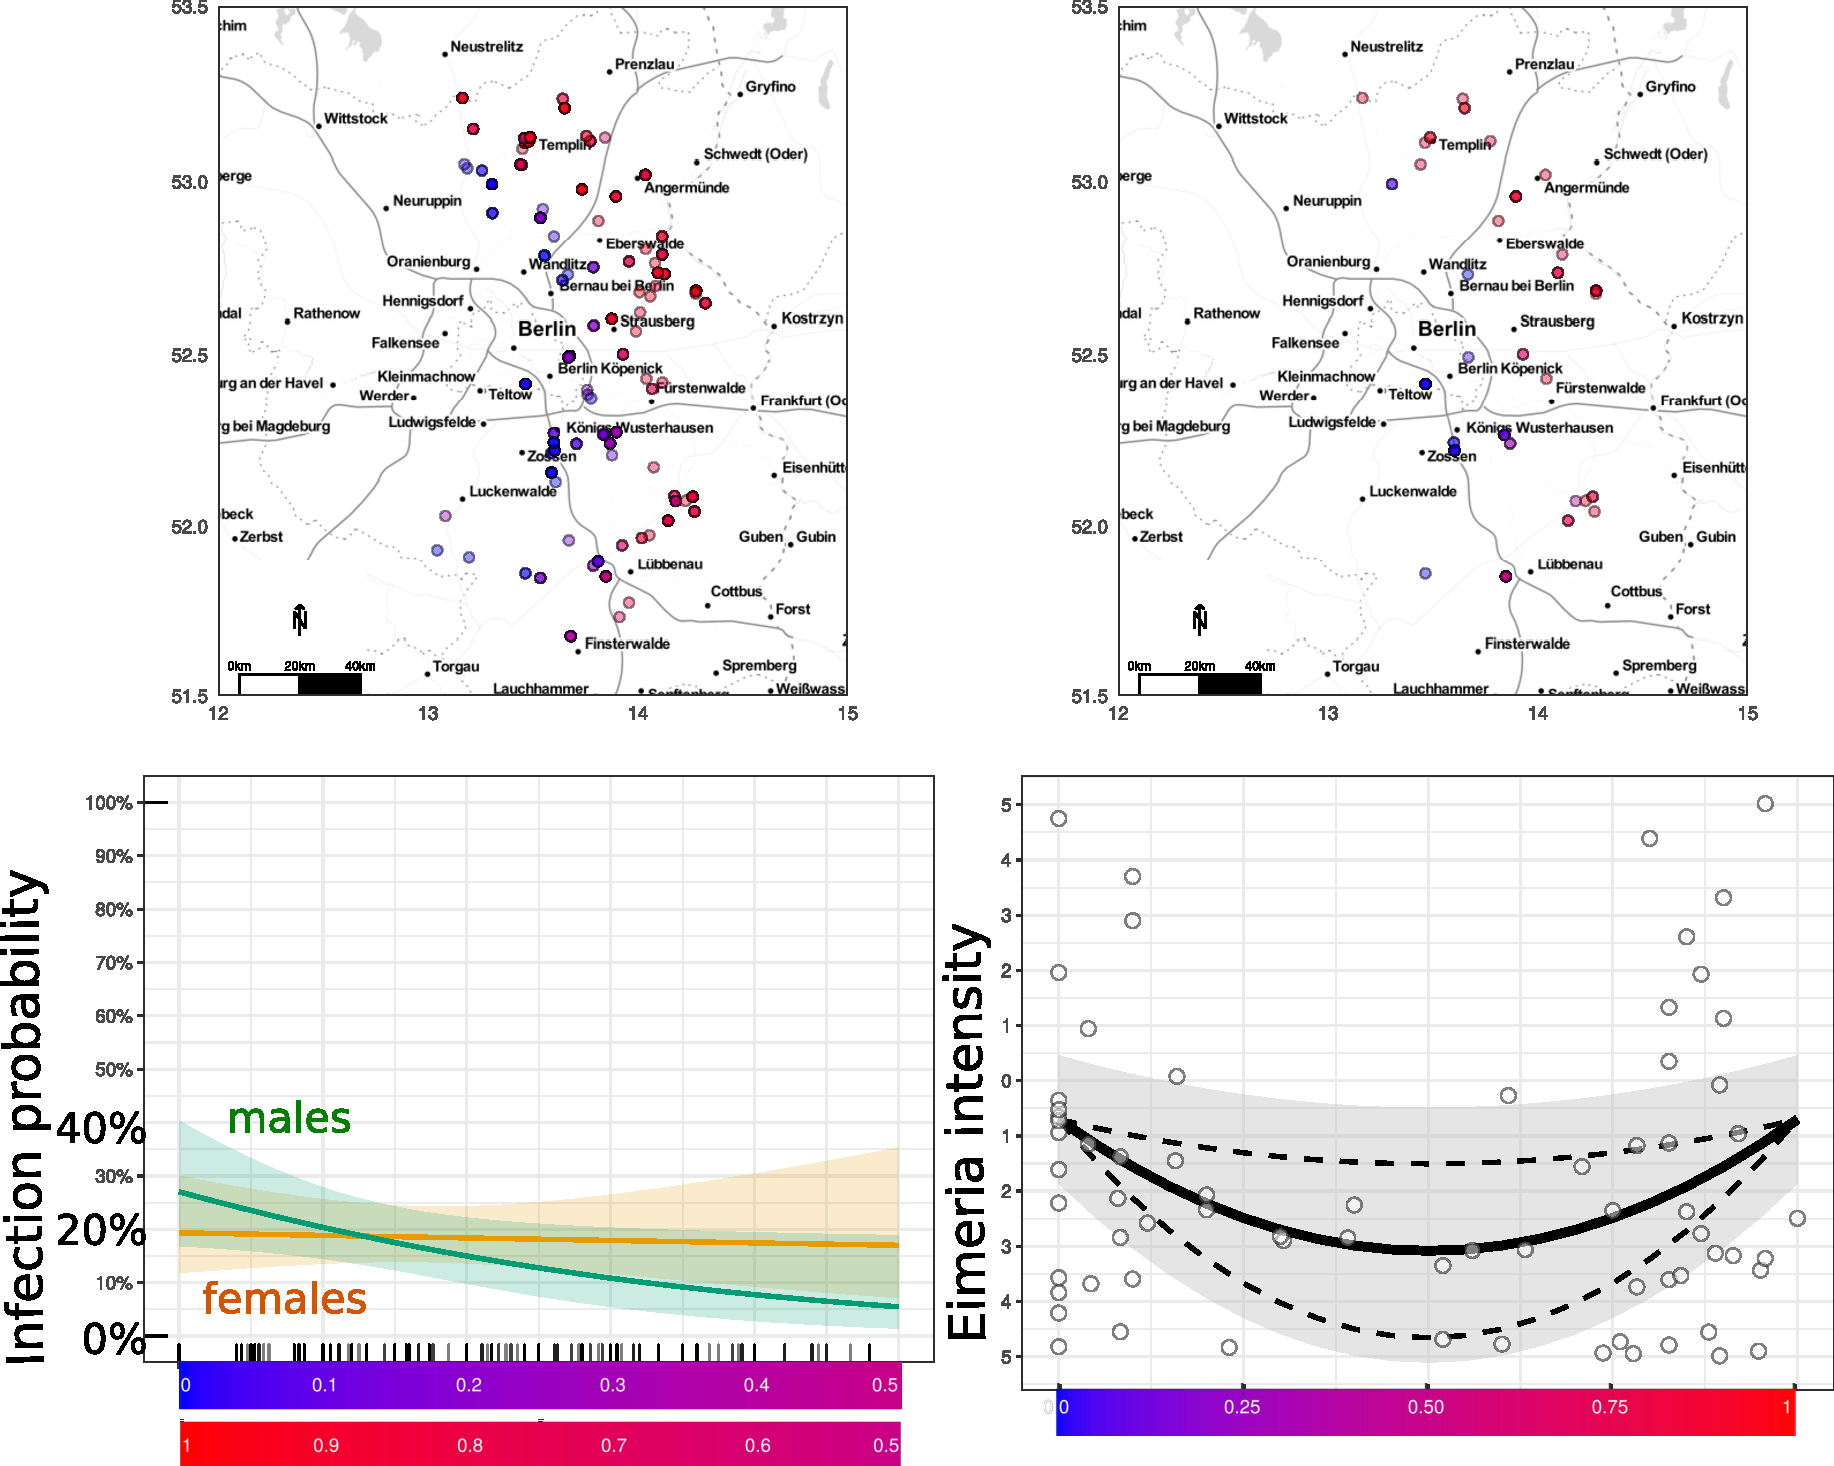
\includegraphics[scale=0.9]{Figure2.pdf}
      \end{tikzfigure}

      \begin{tikzfigure}[Pinworms]
        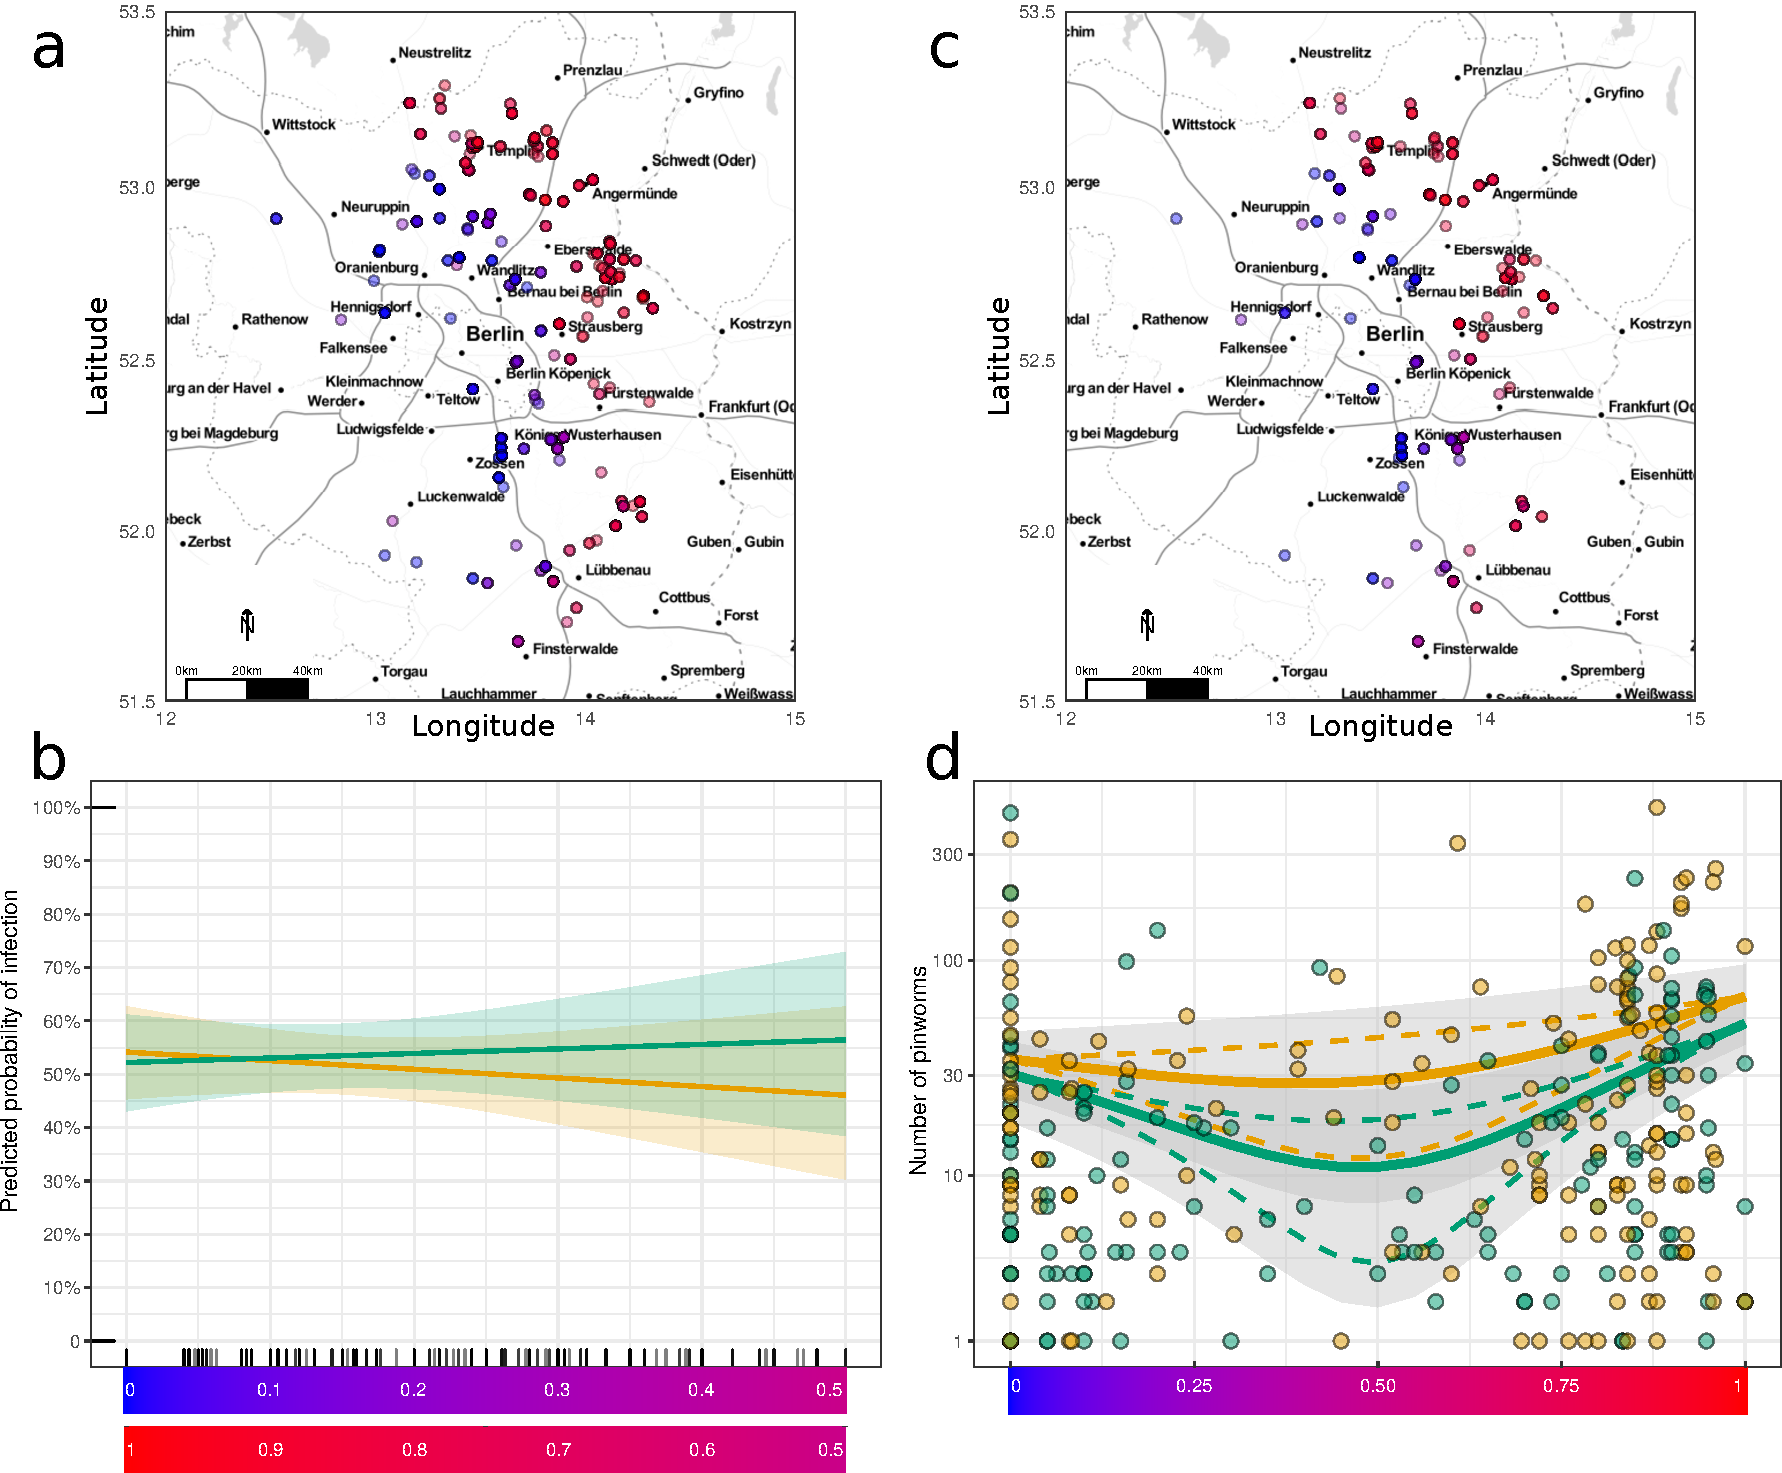
\includegraphics[scale=0.9]{Figure3.pdf}
      \end{tikzfigure}

      \end{multicols*}
(a) Maps of all individuals    (b) Predicted probability of infection when approaching the hybrid zone center \newline
(c) Maps of positive individuals    (d) Prediction of parasite intensity along the hybrid index \newline
males (green)/females (orange)

\begin{itemize}
\item No indication of differential body condition between infected/non infected: no evidence of different impacts on hybrid vs. parental hosts health
\end{itemize}
}

\block{Conclusion}
{

\begin{itemize}
  \item Increased resistance of hybrid mice compared to parental strains for both lower pathogenic parasite (pinworms) and high pathogenic one (Eimeria)
  \item Control for density troughs: no evidence of a lower parasite prevalence in the centre of the hybrid zone (exclude external ecological epidemiological factors)
  \item \textbf{Independance} of hybrid resistance from the parasite pathogenicity level
  
\end{itemize}
}

% REFERENCES
% ----------


\begin{columns} 
  \column{0.65} \block{References}{
Balard \textit{et al.} (unpublished) Reduced Eimeria and pinworms loads in hybrid mice of the European house mouse hybrid zone \newline
R package used for modelling: Balard, A., and E. Heitlinger. 2019. Alicebalard/parasiteLoad DOI: 10.5281/zenodo.2535547
  }
  \column{0.35} \block{}{
    \begin{tikzfigure}[]
      
\includegraphics[scale=0.8]{Logo.png}
    \end{tikzfigure}}
\end{columns}

% ----------------
\end{document}
\endinput
%%
%% End of file 
